We will now examine the more general case of particles with bounded centripetal acceleration, $\abs{a_c(t)} \le \bar{a_c}$, for some $\bar{a_c} \ge 0$. This case is much more relevant to physical problems, because objects typically have momentum which limits their ability to turn quickly. To keep the problem manageable, all particle in this section have zero tangential acceleration, $a_t(t) = 0$, and $v(t) = \bar{v}$.

\begin{lemma} \label{lem:r-curve}
  Given a particle with constant speed and bounded centripetal acceleration, the minimum radius of curvature of the particle's trajectory is given by

  \begin{equation}
    R_{min} = \frac{\bar{v}^2}{\bar{a}_c}
  \end{equation}
  \end{lemma}

\begin{proof}

This comes directly from the definition of radius of curvature for a particle with zero tangential acceleration:

\[
  R(t) = \frac{\bar{v}^2}{a_c(t)}
\]

and 

\[
  a_c(t) \le \bar{a}_c \to \frac{1}{a_c} \ge \frac{1}{\bar{a}_c}
\]
\end{proof}

At the beginning of our paper we mentioned that there is a case when a particle is too close to the ending position and can't turn fast enought, so it ends up passing by it. We formalize this notion in the following lemma.

\begin{lemma}\label{lem:too-close}
  Let particle $p$ have constant speed, bounded centripetal acceleration, an initial angle $\theta_0$, starting position $\bvec{X_0}$, and ending position $\bvec{X_f}$. Every valid path where $\theta(t)$ is minimized for all $t \in [T_0(\bhat{\gamma_p}), T_f(\bhat{\gamma_p})]$ has $d(\bvec{X_0}, \bvec{X_f}) \ge 2 R_{min} \cos\paren{\theta_0}$.
\end{lemma}

\begin{proof}

  The following figure will help illustrate the theorem.

  \begin{figure}[H]
    \begin{center}
      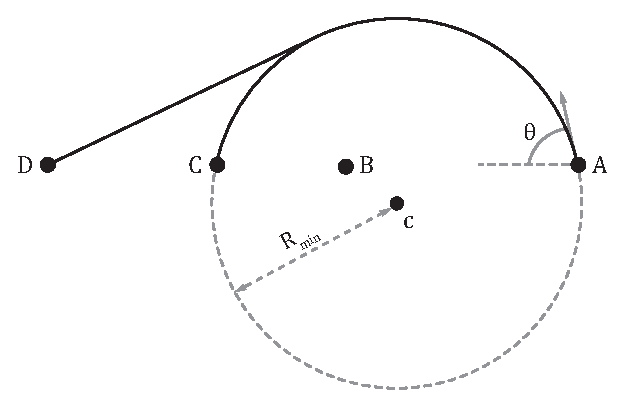
\includegraphics[width=3.5in,height=2.5in,keepaspectratio]{valid_trajs.eps}
    \end{center}
  \vspace{-.2in} % corrects bad spacing
  \caption{\label{fig:valid-traj}}
  \end{figure}

  One should notice that if $X_f$ is any position inside the circle of radius $R_{min}$, such as point B, then the path is invalid. It is not possible to turn inside the circle, because the centripetal acceleration is bounded. Thus, C is the closest valid ending position. C is a distance $2 R_{min} \cos\paren{\theta_0}$ away from A.

\end{proof}

In order to continue, we must first make a conjecture about how fastest paths behave. Unfortunately, our research has not yet yielded a rigorous proof of this conjecture, so we will provide some intuition behind it.

\begin{conjecture}\label{conj:optimal-position}
  Let $p_1, p_2$ be particles with constant speed, bounded centripetal acceleration, starting positions $\bvec{X_1}, \bvec{X_2}$ respectively, and a final position $\bvec{X}_f$, such that $d(\bvec{X_1}, \bvec{X}_f), d(\bvec{X_2}, \bvec{X}_f) \ge 2 R_{min} \cos\paren{\theta_0}$. If $r_1(T_0) \leq r_2(T_0)$ and $\abs{\theta_1(T_0)} < \abs{\theta_1(T_0)}$, then $T_f(\hat{\gamma_1}) < T_f(\hat{\gamma_2})$.
\end{conjecture}

In words, this conjecture states that a particle $p_2$ that is further away from $X_f$ cannot overtake another particle $p_1$ that is closer to $X_f$, if $\theta_1(t) \le \theta_2(t)$. The intuition behind this is that $p_2$ must travel further than $p_1$ to reach $X_f$, because it is further away. Furthermore, one could also imagine, that if this conjecture were not true, then it would be fastest to move away from $X_f$ for some period of time, which seems intuitively wrong.

The special case when $d(\bvec{X_1}, \bvec{X}_f), d(\bvec{X_2}, \bvec{X}_f) < (1/2) R_{min} \cos\paren{\theta_0}$ is omitted, because some special strategy will be needed in this situation. We leave this case as an open problem in our paper. 

Assuming that Conjecture \ref{conj:optimal-position} is true, we will move on to prove one final theorem about fastest paths.

\begin{theorem}
  Let  $p$ be a particle with constant speed, bounded centripetal acceleration, initial angle $\theta_0$, starting position $\bvec{X}_0$, and ending position $\bvec{X}_f$, such that $d(\bvec{X}_0, \bvec{X}_f) \ge 2 R_{min} \cos\paren{\theta_0}$. The unique fastest path $\bhat{\gamma_p}$ for particle $p$ to reach $\bvec{X}_f$ minimizes $\theta(t)$ for all $t \in [T_0(\bhat{\gamma_p}), T_f(\bhat{\gamma_p})]$.
  \label{thm:restricted-theta}
\end{theorem}
\begin{proof}
Let $p_1$ be a particle whose path $\gamma_1$ minimizes $\abs{\theta_1(t)}$ for all times $t \in [T_0(\gamma_1), T_f(\gamma_1)]$. We shall show that $\gamma_1$ is the unique fastest path.

Let $t_s$ be the smallest time such that $\theta_p(t) = 0$. From \ref{thm:theta-min}, we know that $\theta_p(t) = 0$ for $t \ge t_s$, so the particle moves in a straight line towards $X_f$ for $t \ge t_s$. To show that $\gamma_1(t)$ truly is a fastest path, we must examine what happens for $t < t_s$.

We know that $\abs{a_{c,1}(t)} = \bar{a}_c$ for all $t < t_s$ because $p_1$ follows a path that minimizes $\abs{\theta_1(t)}$.

Now let us introduce a particle $p_2$ with the same conditions as $p_1$, but different centripetal acceleration. For some small enough $\epsilon > 0$, we can now find a time interval $t \in [t_b-\epsilon, t_b+\epsilon]$ where that $a_{c,2}(t) < a_{c,1}$.  We shall show that the fastest path for $p_2$, $\hat{\gamma_2(t)}$, after $t_b$ is strictly worse than the fastest path for $p_1$, $\hat{\gamma}_1$, which will allow us to conclude that $\gamma_1(t)$ is the unique fastest path.

Because $\gamma_1$ minimizes $\abs{\theta(t)}$, $\abs{\theta_1(t_b)} \le \abs{\theta_2(t_b)}$. If $t_b > t_s$, then from \ref{thm:theta-min} we know that $\gamma_2(t)$ is worse than $\gamma_1$. If $t_b \le t_s$, we will prove that $r_1(t_b) < r_2(t_b)$. 

Looking at Equation \ref{eq:r-diff}

\begin{align*}
  r(t_b)& = r(t_b-\epsilon) - \bar{v} \int_{t' = T_0}^{t} \cos(\abs{\theta(t')}) dt'
\end{align*}

Since $\cos(\abs{\theta_1(t)}) \ge \cos(\abs{\theta_2(t)})$, $r_1(t_b) \le r_2(t_b)$, so we can invoke Conjecture \ref{conj:optimal-position} to show that $\gamma_1$ is a fastest path which finishes the proof.
\end{proof}